\documentclass[11pt]{article}
\usepackage[margin=1in]{geometry}
\usepackage{booktabs,graphicx,amsmath}
\title{Online Q on a short-horizon control task\\
\large The share is a state, not a penalty on a menu}
\author{}
\date{}
\begin{document}
\maketitle

\section{The scenario}

The scorecard race picks one frozen score for a batch of 200 rows. A
constant-step update of that menu is a stateless bandit, and a step size
\(1/n\) is the sample mean already inside UCB. This note changes the decision.

Each round is an episode of four steps on 200 trajectories drawn from the
pool. The action is \(-1\), \(0\), or \(+1\). The state moves by
\(s\leftarrow 0.85 s + 0.15 a v\), with \(v\) the unit vector, and the reward is
\(a(s^\top\beta_t)-0.05 a^2\) plus \(N(0,0.25^2)\) noise. There is no discount.
The coefficient \(\beta_t\) follows the same gradual ramp as the relocation MVP:
it stays on the first block through round 20, then moves linearly onto the
second block. A second run flips the sign of the first block on that same
ramp. The next round is not announced, and there is no jump.

The observable state for Q is the three-way sign of two known reference
scores, \(s^\top\beta_A\) and \(s^\top\beta_B\), and the step index. Nine
cells times four steps. On a sign flip the second score is the negative of
the first, so the cell does not by itself say which sign is live. A second
set of tables also conditions on which of the four reference policies
currently holds the pseudo-outcome share. The share uses the fixed calendar
from the scorecard race: the first six rounds against the latest six, refreshed
every eight rounds from round 16. Until that refresh the share bin is empty.
Reference policies are scored on every batch, as the scorecards were.

The baseline commits to one reference policy for the whole episode and picks
it with UCB, discounted UCB, \(\varepsilon=0.10\), or UCB minus \(\eta\sigma w_k\)
at \(\eta=2\). Q is updated once per visited state-action at the end of the
step, with \(\alpha=0.2\), on the average temporal-difference error of the
particles in that cell. Tables start at zero. Greedy Q with no bonus keeps
the first action that breaks the tie. The visit-bonus rules add
\(\sqrt{2\log(t+1)/n}\) at decision time only, with a large bonus on a
cell that has not been visited, and the bonus is not part of the backup.
Double Q keeps two tables, acts on their average plus that same bonus, and
bootstraps from the table that was not updated. Ties are broken by a fresh
jitter, so the first batch spreads its particles across tied actions.

Excess is the noise-free return of the finite-horizon optimum minus the
noise-free return of the actions taken, summed over rounds after the ramp
crosses one half. The optimum is the exact action tree; the dynamics have no
process noise.

\section{Relocation}

UCB at \(\eta=2\) has median post-shift excess
9.7, against
32.7 for plain UCB and
15.3 for discounted UCB.
\(\varepsilon=0.10\) is 53.1.
Greedy Q on the sign state is 39.2.
The same table with the share bin is 21.1.
Q with a visit bonus is 15.9 without the
share and 28.1 with it. Double Q is
21.6 on signs and
38.7 with the share bin.

The visit-bonus table on the two scores, QUCB, is lower than plain UCB by
more than the larger seed standard deviation on
5/6 pools, and lower than UCB at
\(\eta=2\) on 0/6. UCB at
\(\eta=2\) is lower than QUCB on
2/6. Adding the share bin, QS, is
lower than UCB at \(\eta=2\) on 0/6
and higher on 5/6. Greedy Q with no
bonus is lower than UCB at \(\eta=2\) on
0/6. Early excess, before the ramp,
is 12.5 for UCB,
11.9 for the tax,
5.4 for sign-only Q, and
10.4 for the share-bin table.
The post-shift hit rate on the first action is
0.80 for visit-bonus Q and
0.85 for UCB at \(\eta=2\).

\section{Sign flip}

On the sign flip, UCB is 148.3, discounted UCB is
99.2, and UCB at \(\eta=2\) is
132.0. Visit-bonus Q on the two scores is
7.3, and double Q on the same state is
24.2. Greedy Q with no bonus is
81.4. The share-bin table is
62.9, its visit-bonus version is
25.9, and double Q with the share bin is
39.6.

QUCB is lower than discounted UCB by more than the seed standard deviation on
6/6 pools, and lower than UCB at
\(\eta=2\) on 6/6. It is lower than the
share-bin visit-bonus table on 6/6.
Greedy Q with no bonus is lower than discounted UCB on
6/6. The first-action hit rate is
0.63 for QUCB and
0.04 for UCB at \(\eta=2\).

A constant step replaces the action stored in a cell. On a flip the same
score-sign cell needs the opposite action after the ramp, and the visit bonus
is what keeps the other actions available while that replacement happens.
Splitting the cell by the share bin means each piece is visited less often.
The scorecard MVP keeps its index. This note is the record of the control
task, where the decision depends on the current scores.

\begin{table}[ht]
\centering
\caption{Median, across six pools, of the four-seed mean post-shift excess return.}
\resizebox{\textwidth}{!}{%
\begin{tabular}{lcccccccccc}
\toprule
scenario & UCB & DUCB & UCB-H2 & EG10 & Q & QUCB & DQ & QS & QS-UCB & DQS \\
\midrule
control\_relocate & 32.7 & 15.3 & 9.7 & 53.1 & 39.2 & 15.9 & 21.6 & 21.1 & 28.1 & 38.7 \\
control\_flip & 148.3 & 99.2 & 132.0 & 153.1 & 81.4 & 7.3 & 24.2 & 62.9 & 25.9 & 39.6 \\
\bottomrule
\end{tabular}}
\end{table}

\begin{table}[ht]
\centering
\caption{Control relocation. Sum of per-round mean excess return after the ramp crosses one half. Seed standard deviation in parentheses.}
\resizebox{\textwidth}{!}{%
\begin{tabular}{lcccccc}
\toprule
pool & UCB & DUCB & UCB-H2 & QUCB & DQ & QS-UCB \\
\midrule
AR(1) & 31.5 (1.1) & 15.2 (1.4) & 9.8 (4.8) & 9.6 (0.6) & 13.0 (1.5) & 23.5 (0.7) \\
California & 8.6 (0.5) & 6.4 (0.1) & 3.3 (0.2) & 12.5 (0.5) & 9.3 (0.7) & 21.8 (0.7) \\
covertype & 33.9 (4.5) & 14.9 (0.8) & 7.2 (0.3) & 26.2 (3.1) & 28.0 (0.6) & 35.4 (2.7) \\
Gaussian-12 & 30.8 (0.8) & 15.4 (0.4) & 9.5 (2.4) & 9.7 (0.8) & 15.5 (1.0) & 25.5 (0.7) \\
Gaussian-30 & 50.9 (1.4) & 22.9 (1.1) & 20.4 (0.6) & 21.5 (3.3) & 27.7 (2.2) & 30.6 (0.6) \\
Student-$t_5$ & 44.9 (3.2) & 23.5 (1.2) & 19.4 (1.3) & 19.4 (3.0) & 29.4 (2.0) & 31.2 (0.7) \\
\bottomrule
\end{tabular}}
\end{table}

\begin{table}[ht]
\centering
\caption{Control sign flip. Same excess. Seed standard deviation in parentheses.}
\resizebox{\textwidth}{!}{%
\begin{tabular}{lcccccc}
\toprule
pool & UCB & DUCB & UCB-H2 & QUCB & DQ & QS-UCB \\
\midrule
AR(1) & 97.6 (1.0) & 65.3 (1.2) & 88.5 (1.6) & 2.3 (0.8) & 12.1 (3.1) & 15.3 (4.8) \\
California & 83.5 (1.3) & 56.9 (2.2) & 78.2 (1.6) & 2.4 (0.6) & 10.3 (1.9) & 10.6 (5.5) \\
covertype & 200.4 (3.6) & 132.9 (1.9) & 160.9 (7.4) & 22.8 (10.6) & 37.7 (5.8) & 43.2 (6.5) \\
Gaussian-12 & 115.1 (2.9) & 78.8 (1.3) & 105.5 (3.6) & 2.9 (0.5) & 16.8 (2.4) & 20.5 (4.5) \\
Gaussian-30 & 185.6 (3.1) & 124.9 (3.5) & 160.4 (7.1) & 12.6 (5.3) & 31.6 (4.3) & 37.3 (11.5) \\
Student-$t_5$ & 181.5 (1.4) & 119.6 (3.7) & 158.5 (4.9) & 11.6 (7.0) & 34.8 (6.6) & 31.3 (15.4) \\
\bottomrule
\end{tabular}}
\end{table}


\begin{figure}[ht]
\centering
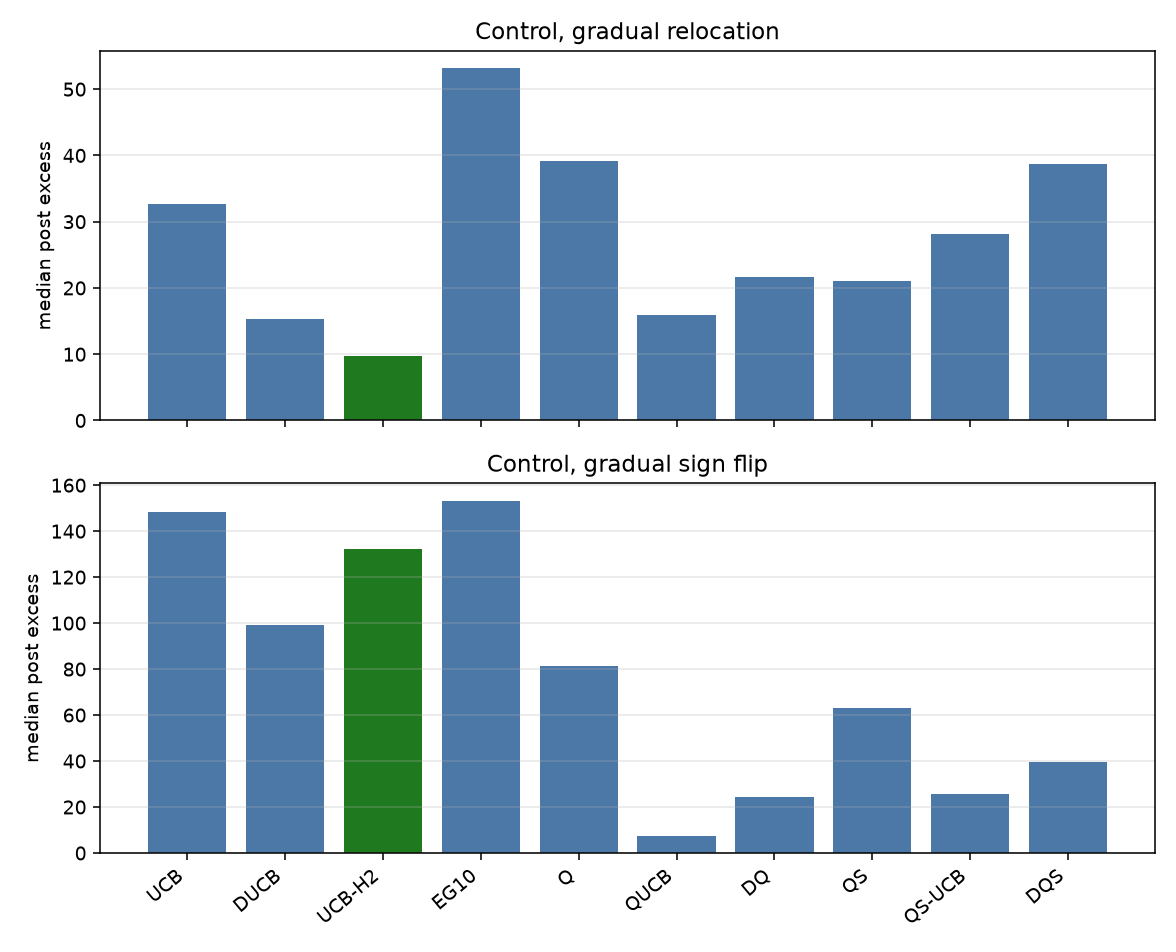
\includegraphics[width=\textwidth]{control_bars.png}
\caption{Median post-shift excess return across six pools.
UCB at \(\eta=2\) is marked in green. The top panel relocates the reward
block. The bottom panel flips its sign.}
\end{figure}
\end{document}
